\documentclass{article}
\usepackage[utf8]{inputenc}
\usepackage{amsmath}
\usepackage{amssymb}
\usepackage{comment}
\usepackage{graphicx}
\usepackage{amsfonts}
\usepackage{float}
\title{Assignment 5 - Solutions of Problems on Logic}
\begin{document}
\maketitle
\begin{enumerate}

\item The cafe in-charge gets 2 cups of coffee, one for Prof. Puneet and one for Prof. Apurva. \\ 
The in-charge concludes this from the fact that - in case Puneet did not want coffee, he would have definitely answered a "No". Given that his response was "I don't know" is indicative of the fact that he is interested but is unsure of others. Similar is the case with Apurva, who is unsure of Nittin's choice. Finally, when Nittin says "No", it is indicative of the fact that he is not interested in having coffee.

\item The below table captures the equivalence of the given statements:
\begin{figure}[H]
\centering
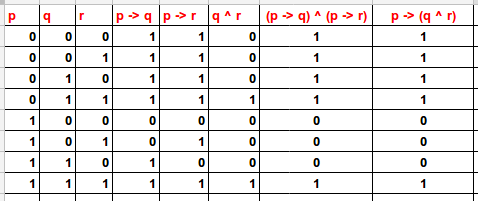
\includegraphics[width = 10cm]{truth_table}
\end{figure}

\item Let $n \in \mathbb{Z}^+$, we need to show that $\overline{v_1 + v_2 + \dots v_n} = \overline{v_1}. \overline{v_2}. \dots \overline{v_n}$\\

We prove the following through induction. \\
Let the base case be proved for the case when $n=2$, which directly follows from the DeMorgan's Law. \\ 
Let us assume this is true up to $k$ variables (induction hypothesis), i.e  $\overline{v_1+v_2+ \dots v_k} = \overline{v_1}. \overline{v_2}. \dots \overline{v_k}$\\
Given the induction hypothesis, we prove that the statement is true for $k+1$ variables as well.\\
\begin{align*}
\overline{v_1+v_2+ \dots v_k+v_{k+1}} & = \overline{(v_1+v_2+ \dots v_k)+v_{k+1}} \\ 
& = \overline{v_1+v_2+ \dots v_k}~.~\overline{v_{k+1}}\\
&= \overline{v_1}~.~ \overline{v_2}~.~ \dots \overline{v_k}~.~ \overline{v_{k+1}}
\end{align*}
The last step follows from the induction hypothesis.\\
A very similar argument can be made to prove $\overline{v_1~.~ v_2 ~.~ \dots v_n} = \overline{v_1}~+~ \overline{v_2}~+~ \dots \overline{v_n}$

\item A propositional statement is \textit{satisfiable} if and only if, its truth table is not a \textit{contradiction}. The example in the previous question was one such example : $(p\rightarrow q)\wedge(p\rightarrow r)$.


\item Yes. One can conclude this by writing the truth table for the same. However, let us look at the possibility of the proposition being False. $a \rightarrow b$ is False only when $a$ is True and $b$ is false. Hence, for the given proposition to be False, we know the truth vale of $p$ must be True. Similarly we can argue for $q$ to be True. Evaluating the proposition for these truth values, we can conclude that the proposition is always True and hence a \textit{tautology}.


\item The proposition is neither a \textit{contradiction} nor a \textit{tautology}. We conclude this by evaluating the statement for the truth values $q=T;p=F$ and $q=0;p=0$.

\item Listed below is the steps and the reason
\begin{center}
\begin{tabular}{ l l }
 (1)~$\lnot (\lnot q \rightarrow s)$ & Negation of the conclusion \\ 
 (2)~$\lnot q \wedge \lnot s$ & Step (1) and $\lnot q \wedge \lnot s \leftrightarrow \lnot(\lnot\lnot q \vee s)$  \\  
 (3)~$\lnot s$ & Step (2) and the Rule of Conjunctive Simplification \\ 
 (4)~$\lnot r  \vee s$ & Premise  \\ 
 (5)~$\lnot r $ & Step (3),(4) and the Rule of Disjunctive Syllogism  \\  
 (6)~$p \rightarrow q$ & Premise  \\
 (7)~$\lnot q$ & Step (2) and the Rule of Conjunctive Simplification  \\ 
 (8)~$\lnot p$ & Step (6),(7) and Rule of Modes Tollens  \\  
 (9)~$p \vee r$ & Premise  \\
 (10)~$r$ & Step (8),(9) and the Rule of Disjunctive Syllogism   \\
 (11)~$\lnot r \wedge r$ & Step (5),(10) and the Rule of Conjunction  \\
 (12)~$\therefore \lnot q \rightarrow s$ & Step (11) and Proof by Contradiction   
\end{tabular}
\end{center}

\item Below is the arguments in the symbolic form :

\begin{enumerate}

\item $p:$ Reshma gets the supervisor’s position\\
$q:$ Reshma works hard \\ 
$r:$ Reshma gets a raise \\ 
$s:$ Reshma buys a new car\\

$(p \wedge q) \rightarrow r$\\
$r \rightarrow s$\\
$\lnot s$\\ 
-------------\\
$\therefore \lnot p \vee \lnot q$\\ 

\begin{center}
\begin{tabular}{ l l }
(1)~$\lnot s$ & Premise \\
(2)~$r \rightarrow s$ & Premise  \\ 
(3)~$\lnot r$ & Steps (1),(2) and Modus Tollens \\
(4)~$(p \wedge q) \rightarrow r$ &  Premise \\ 
(5)~$\lnot(p \wedge q)$ & Steps (3),(4) and Modus Tollens  \\
(6)~$\therefore  \lnot p \vee \lnot q$ & Step (5) and $\lnot (p \wedge q) \leftrightarrow \lnot p \vee \lnot q$    
\end{tabular}
\end{center}


\item $p:$ Dinesh goes to the racetrack\\
$q:$ Hema gets mad \\ 
$r:$ Ravi plays card all night \\ 
$s:$ Cinderella gets mad\\
$t:$ Veena is notified\\

$p \rightarrow q$\\
$r \rightarrow s$\\
$(q \vee s) \rightarrow t$\\ 
$\lnot t$\\ 	
-------------\\
$\therefore \lnot p \wedge \lnot r$\\

\begin{center}
\begin{tabular}{ l l }
(1)~$\lnot t $ & Premise \\  
(2)~$(q \vee s) \rightarrow t $ & Premise\\  
(3)~$ \lnot(q \vee s) $ & Steps (1),(2) and Modus Tollens \\  
(4)~$\lnot q \wedge \lnot s $ & Step (3) and DeMorgan's Law\\  
(5)~$ \lnot q $ & Step (2) and the Rule of Conjunctive Simplification \\  
(6)~$p \rightarrow q $ & Premise\\  
(7)~$ \lnot p$ & Steps (5),(6) and Modus Tollens \\
(8)~$\lnot s $ & Step (4) and the Rule of Conjunctive Simplification \\  
(9)~$r \rightarrow s $ & Premise\\  
(10)~$\lnot r $ & Steps (8),(9) and Modus Tollens \\ 
(11)~$\therefore \lnot p \wedge \lnot r $ & Step (7),(10) and rule of Conjunction\\  
\end{tabular}
\end{center}
\end{enumerate}


\item For the statement to not be Tautology, there must be some assignment of truth values to the variable so that the statements evaluates to a False. In order to see if such an assignment exists, we know that the expression $(q \vee r)$ must be False while $(p \vee q) \wedge (\lnot p \vee r)$ must be True. This is the only case when the given proposition will evaluate to a False. \\

If $(q \vee r)$ is False then the only assignments of the variables are $q=F;r=F$. Given this, we can now reduce the left hand side expression as $(p \vee F) \wedge (\lnot p \vee F) \implies (p \wedge \lnot p) \implies F$. This shows that there is no assignment that can make the proposition False. Hence it is a tautology.

\begin{enumerate}
\item Below we provide the steps and the reason:
\begin{center}
\begin{tabular}{ l l }
(1)~$p \vee (q \wedge r)$ & Premise \\ 
(2)~$(p \vee q) \wedge (p \vee r)$ & Step (1) and the Distribution Law \\ 
(3)~$p \vee r$ & Step (2) and the Rule of Conjunctive Simplification \\ 
(4)~$p \rightarrow s$ & Premise \\ 
(5)~$\lnot p \vee s$ & Step (4), $p \rightarrow s \leftrightarrow (\lnot p \vee s)$ \\ 
(6)~$\therefore r \vee s$ & Step (3),(5), Rule of Conjunction, and Resolution 
\end{tabular}
\end{center}


\item Below we provide the steps and the reason:
\begin{center}
\begin{tabular}{ l l }
(1)~$\lnot p \vee s$ & Premise\\ 
(2)~$p \vee q\vee t $ & Premise\\
(3)~$p \vee (q\vee t) $ & Step (2) and Associative Law\\
(4)~$[[p \vee (q\vee t)]\wedge (\lnot p \vee s) ] $ & Step (3)(1) and Rule of Conjunction\\
(5)~$(q \vee t)\vee s $ & Step (4) and Resolution\\
(6)~$q \vee (t\vee s) $ & Step (5) and Associative law \\
(7)~$\lnot q \vee r $ & Premise \\
(8)~$[[q \vee (t\vee s)]\wedge [\lnot q \vee r]] $ & Step (6)(7) and Rule of Conjunction\\
(9)~$(t\vee s)\vee r $ & Step (8) and Resolution\\
(10)~$t\vee (s\vee r) $ & Step (9) and Associative law \\
(11)~$\lnot t\vee (s\vee r)  $ & Premise\\
(12)~$(\lnot t\vee s) \wedge (\lnot t\vee r) $ & Step (11) and Distributive law\\
(13)~$\lnot t\vee s $ & Step (12) and Rule of Conjunction Simplification\\
(14)~$[[t\vee (s\vee r)]\wedge (\lnot t\vee s)] $ & Step (10)(13) and Rule of Conjunction \\
(15)~$(s \vee r) \vee s $ &  Step (14) and Resolution\\
(16)~$\therefore r \vee s $ & Step (15) and Commutative, Associative and Idempotent Laws of $\vee$
\end{tabular}
\end{center}
\end{enumerate}

\item $p:$ Jonathan has a driver's license\\
$q:$ Jonathan's new car is out of gas \\ 
$r:$ Jonathan likes to drive his new car\\ 

Then the given argument can be written as follows:\\
$\lnot p \vee q$\\
$p \vee \lnot r$\\
$\lnot q \vee \lnot r$\\ 	
-------------\\
$\therefore \lnot r$\\

\begin{center}
\begin{tabular}{ l l }
(1)~$\lnot p \vee q $ & Premise \\  
(2)~$p \vee \lnot r $ & Premise\\ 
(3)~$(\lnot p \vee q)\wedge (p \vee \lnot r) $ & Step (1)(2) and Rule of Conjunction\\ 
(4)~$\lnot r \vee q $ & Step (3) and Resolution \\ 
(5)~$q \vee \lnot r $ & Step (4) and Commutative Law\\ 
(6)~$\lnot q \vee \lnot r $ & Premise\\ 
(7)~$(q \vee \lnot r) \wedge (\lnot q \vee \lnot r) $ & Step (5)(6) and rule of Conjunction\\ 
(8)~$\lnot r \vee \lnot r $ & Step (7) and Resolution \\ 
(9)~$\therefore \lnot r $ & Step (8) and Idempotent Law \\ 
\end{tabular}
\end{center}

\item Below are the truth values for each of the statements:
\begin{enumerate}
\item True
\item False
\item False
\item True
\end{enumerate}
\end{enumerate}



\end{document}
